\section{Eliminating Timing Side-Channel-Attacks}
\label{sec:app_side_channel_attack}

Encryption algorithms are based on strong mathematical properties to prevent attackers from deciphering the encrypted content. 
%only timing attacks
However, their implementations in software naturally introduce varying run times because of data-dependent control flow paths.
Timing attacks~\cite{Kocher96timingattacks} exploit this variability in cryptosystems and extract additional information  from executions of the cipher.
These can lead to deciphering the secret key.
Kocher describes a timing attack as a basic signal detection problem~\cite{Kocher96timingattacks}. 
The ``signal'' is the timing variation caused by the key's bits when running the cipher, while ``noise'' is the measurement inaccuracy and timing variations from other factors such as architecture unpredictability and multitasking. 
This signal to noise ratio determines the number of samples required for the attack---the greater the ``noise,'' the more difficult the attack. 
It was generally conceived that this ``noise'' effectively masked the ``signal,'' thereby shielding encryption systems from timing attacks. 
However, practical implementations of the attack have since been presented~\cite{remoteattackspracticle,DKLMQW98,SCAsurvey} that clearly indicate the ``noise'' by itself is insufficient protection. 
In fact, the architectural unpredictability that was initially believed to prevent timing attacks was discovered to enable even more attacks.
Computer architects use caches, branch predictors and complex pipelines to improve the average-case performance while keeping these optimizations invisible to the programmer.
These enhancements, however, result in unpredictable and uncontrollable timing behaviors, which are all shown to be vulnerabilities that lead to side-channel attacks~\cite{2004-bernstein-cachetiming,Percival05cachemissing,Onur07predictingsecret,2009-x86timing}.

In order to not be confused with Kocher's~\cite{Kocher96timingattacks} terminology of \textit{timing attacks} on algorithmic timing differences, we classify all above attacks that exploit the timing variability of software implementation \textit{or} hardware architectures as \textit{time-exploiting attacks}. 
In our case, a \textit{timing attack} is only one possible \textit{time-exploiting attack}.
Other time-exploiting attacks include branch predictor, and cache attacks.
Examples of other side-channel attacks are power attacks~\cite{Messerges99investigationsof,Kocher99differentialpower}, fault injection attacks~\cite{biham97differential,Feng_efficientcomb}, and many others~\cite{SCAsurvey}.
%Bernstein at al.\cite{2004-bernstein-cachetiming} introduced the vulnerabilities of caches to side channel attacks; Aciicmez at al.\cite{Onur07predictingsecret} showed us how the branch predictor could be used as a side channel; 

%Attackers take advantage of different properties of the implementation such as run time, power usage, and even the behavior after manually injecting faults into the system's operation. 

In recent years, we have seen a tremendous effort to discover and counteract side-channel attacks on encryption systems~\cite{biham97differential,2009-x86timing,99designprinciples,fbscc,branchpredict,Kelsey98sidechannel,blindingrsa,cachepartition,sidechannelprocarch}.
However, it is difficult to be fully assured that all possible vulnerabilities  have been discovered.
The plethora of research on side-channel exploits~\cite{2009-x86timing,biham97differential,99designprinciples,fbscc,branchpredict,Kelsey98sidechannel,blindingrsa,cachepartition,sidechannelprocarch} indicate that we do not have the complete set of solutions, as more vulnerabilities are still being discovered and exploited.
Just recently, Coppens et al.~\cite{2009-x86timing} discovered two previously unknown time-exploiting attacks on modern x86 processors caused by the out-of-order execution and the variable latency instructions.
This suggests that while current prevention methods are effective at \textit{defending} against their particular attacks, they do not \textit{prevent} other attacks from occurring.
This, we believe, is because they do not address the root cause of time-exploiting attacks, which is that run time variability \textit{cannot be controlled} by the programmer.

It is important to understand that the main reason for time-exploiting attacks is \textit{not} that the program runs in a varying amount of time, but that this variability \textit{cannot be controlled} by the programmer. 
The subtle difference is that if timing variability is introduced in a controlled manner, then it is still possible to control the timing information that is leaked during execution, which can be effective against time-exploiting attacks. 
However, because of the programmer's \textit{lack of control} over these timing information leaks in modern architectures, noise injection techniques are widely adopted in attempt to make the attack infeasible.
These include adding random delays~\cite{Kocher96timingattacks} or blinding signatures~\cite{Kocher96timingattacks,blindingrsa}. 
Other techniques such as branch equalization~\cite{Molnar05theprogram,SCAsurvey} use software techniques to rewrite algorithms such that they take equal time to execute during each conditional branch. 
We take a different approach to directly address the crux of the problem, which is the \textit{lack of control} over timing behaviors in software.
By using the PRET architecture, designed to allow predictable and controllable timing behaviors, we prevent the attacker from exploiting uncontrollable timing side-channel leaks from the architecture.   
%Computer architects have introduced caches and complex pipelines to improve the average-case performance while keeping these optimizations invisible to the programmer. 
%However, these improvements often attribute to the unpredictable and uncontrollable timing behaviors, which result in time-exploiting attacks.


%By proposing a predictable architecture, it may seem that we are making the attacker's job easier by reducing the ``noise''

At first it may seem that a predictable architecture makes the attacker's task simpler, because it reduces the amount of ``noise'' emitted from the underlying architecture.
However, we contend that in order for timing behaviors to be controllable, the underlying architecture \textit{must} be predictable.
This is because it is meaningless to specify any timing semantics in software if the underlying architecture is unable to honor them.
And in order to guarantee the execution of the timing specifications, the architecture must be predictable. 
%Hiren - I removed this because it was said at the very end of the introduction
%we argue that a combination of software techniques to control execution times, and hardware techniques that make an architecture predictable are necessary to thwart time-exploiting attacks.
%\textcolor{red}{\FIXME{Sounds too casual -- rephrase}Let us also not forget that the architecture unpredictability which was once thought to shield systems from timing attacks were eventually discovered to be the main vulnerabilities in other side-channel attacks, mainly because they were uncontrollable.}
Our approach does not attempt to increase the difficulty in performing time-exploiting attacks, but to eliminate them completely. 
%As such, we argue that only by providing a timing predictable architecture, can we allow controllable timing behaviors, which removes the source of time-exploiting attacks. 

For this application, we present the PRET architecture in the context of embedded cryptosystems, and show that an architecture designed for predictability and controllability effectively eliminates all time-exploiting attacks.
%The PREcision Timed architecture~\cite{pret_cases08} (PRET) allows for precision timing control, and was originally proposed for real-time embedded systems.
%Originally proposed by Lickly et al~\cite{pret_cases08}, PRET provides instruction-set architecture (ISA) extensions that allow programmers to control an algorithm's temporal properties at the software level.
%To guarantee that the timing specifications are honored, PRET provides a predictable architecture that replaces complex pipelines and speculation units with multithread-interleaved pipelines, and replaces caches with software-managed fast access memories.  
%This allows PRET to maintain predictability without sacrificing performance.
We target embedded applications such as smartcard readers~\cite{99designprinciples}, key-card gates~\cite{rfidcrypto}, set-top boxes~\cite{99designprinciples}, and thumbpods~\cite{schaumont2003tts}, which are a good fit for the PRET architecture's embedded nature.
We demonstrate the effectiveness of our approach by running both the RSA and DSA~\cite{dss} encryption algorithms on the PRET architecture, and show its immunity against time-exploiting attacks.
%The combination of ISA extensions and architectural design decision ensures that PRET can provide controllable timing semantics in software, which eliminate the vulnerability of time-exploiting attacks. 
%This makes it an appropriate match for cryptosystems.
This work shows that a disciplined defense against time-exploiting attacks requires a combination of software and hardware techniques that ensure controllability and predictability.

\subsection{Background}
% 1 - 1.5 page
Kocher outlines a notion of timing attacks~\cite{Kocher96timingattacks} on encryption algorithms such as RSA and DSS that require a large number of plaintext-ciphertext pairs and a detailed knowledge of the target implementation.  
By simulating the target system with predicted keys, and measuring the run time to perform the private key operations, the actual key can be derived one bit at a time.
Kocher also introduced power attacks~\cite{Messerges99investigationsof,Kocher99differentialpower}, which use the varying power consumption of the processor to infer the activity of the encryption software over time. 
These played a large role in stimulating research in side-channel cryptanalysis~\cite{mmthesis,Kelsey98sidechannel}, which also found side-channel attacks against IDEA, RC5 and blowfish~\cite{Kelsey98sidechannel}. 
Fault-based attacks~\cite{biham97differential,fbscc,Feng_efficientcomb} were introduced by Bihan et al.~\cite{biham97differential}.
These attacks attempt to extract keys by observing the system behavior to generated faults.
For the side-channel attacks that we have missed, Zhou~\cite{SCAsurvey} presents a survey on a wide range of side-channel attacks.

Dhem et al.~\cite{DKLMQW98} demonstrate a practical implementation of timing attacks on RSA for smart cards and the ability to obtain a 512-bit key in a reasonable amount of time.
Several software solutions such as RSA blinding~\cite{Kocher96timingattacks,blindingrsa}, execution time padding~\cite{Kocher96timingattacks}, and adding random delays~\cite{Kocher96timingattacks} have been proposed as possible defenses against this attack. 
However, these solutions were not widely adopted by the general public until Brumley et al.~\cite{remoteattackspracticle} orchestrated a successful timing attack over the local network on an OpenSSL-based web server.
This motivated further research on timing attacks for other encryption algorithms such as ECC~\cite{Feng_efficientcomb} and AES~\cite{2004-bernstein-cachetiming}.
In particular, Bernstien's attack on AES~\cite{2004-bernstein-cachetiming} targeted the the run time variance of caches.
The introduction of simultaneous multi-threading (SMT) architectures escalated this type of attack on shared hardware components. 
Percival~\cite{Percival05cachemissing} showed a different caching attack method on SMT, made possible because caches were shared by all processes running on the hardware architecture. 
Ac�i�mez et al. introduced branch predictor
attacks~\cite{Onur07predictingsecret,branchpredict} that monitor control flow by
occupying a shared branched predictor. Compiler and source-to-source transformation techniques~\cite{2009-x86timing,Molnar05theprogram} have also been developed to thwart side-channel attacks.

Wang et al.~\cite{sidechannelprocarch} identified the causes of the timing attacks to be the underlying hardware. 
In particular, their work focuses on specialized cache designs, such as Partition-Locked Caches~\cite{cachepartition} and Random Permutation caches~\cite{sidechannelprocarch} that defend against caching attacks in hardware.
Very recently, Coppens~\cite{2009-x86timing} discovered two previously unknown attacks on the complex pipeline run time variance of x86 architectures.

Our work builds upon the experiences of these.
Most solutions employ either exclusively hardware or software techniques to defend against attacks.
We recognize that a complete solution to control temporal semantics requires a combination of both software and hardware approaches to defend against and prevent future side-channel attacks.
Hence, we present an effort that includes timing control instructions to control execution times in software, and a predictable processor architecture to realize the instructions. 
By doing this, we completely eliminate the source of leaked information used by time-exploiting attacks, rendering the system immune against such attacks.
%We now explain in more detail the architecture of PRET in the context of cryptosystems.

%The architectural design of PRET is to allow: 1) better meaning of deadline instructions, 2) you need predictable underlying hardware, 3) which means timing behaviors of threads must be decoupled. 

% PRET is designed to provide controllable timing behaviors.
% This properties has proved to be of critical importance to real-time systems~\cite{pret_cases08}, and time-exploiting attacks have shown that they are just as critical for security systems.
% We present the PRET architecture in detail in the context of time-exploiting attacks.
%This is because PRET eliminates the source of time exploiting attacks, which is the unpredictability and uncontrollability prevalent in modern computer architectures.

%% \begin{figure}
%%   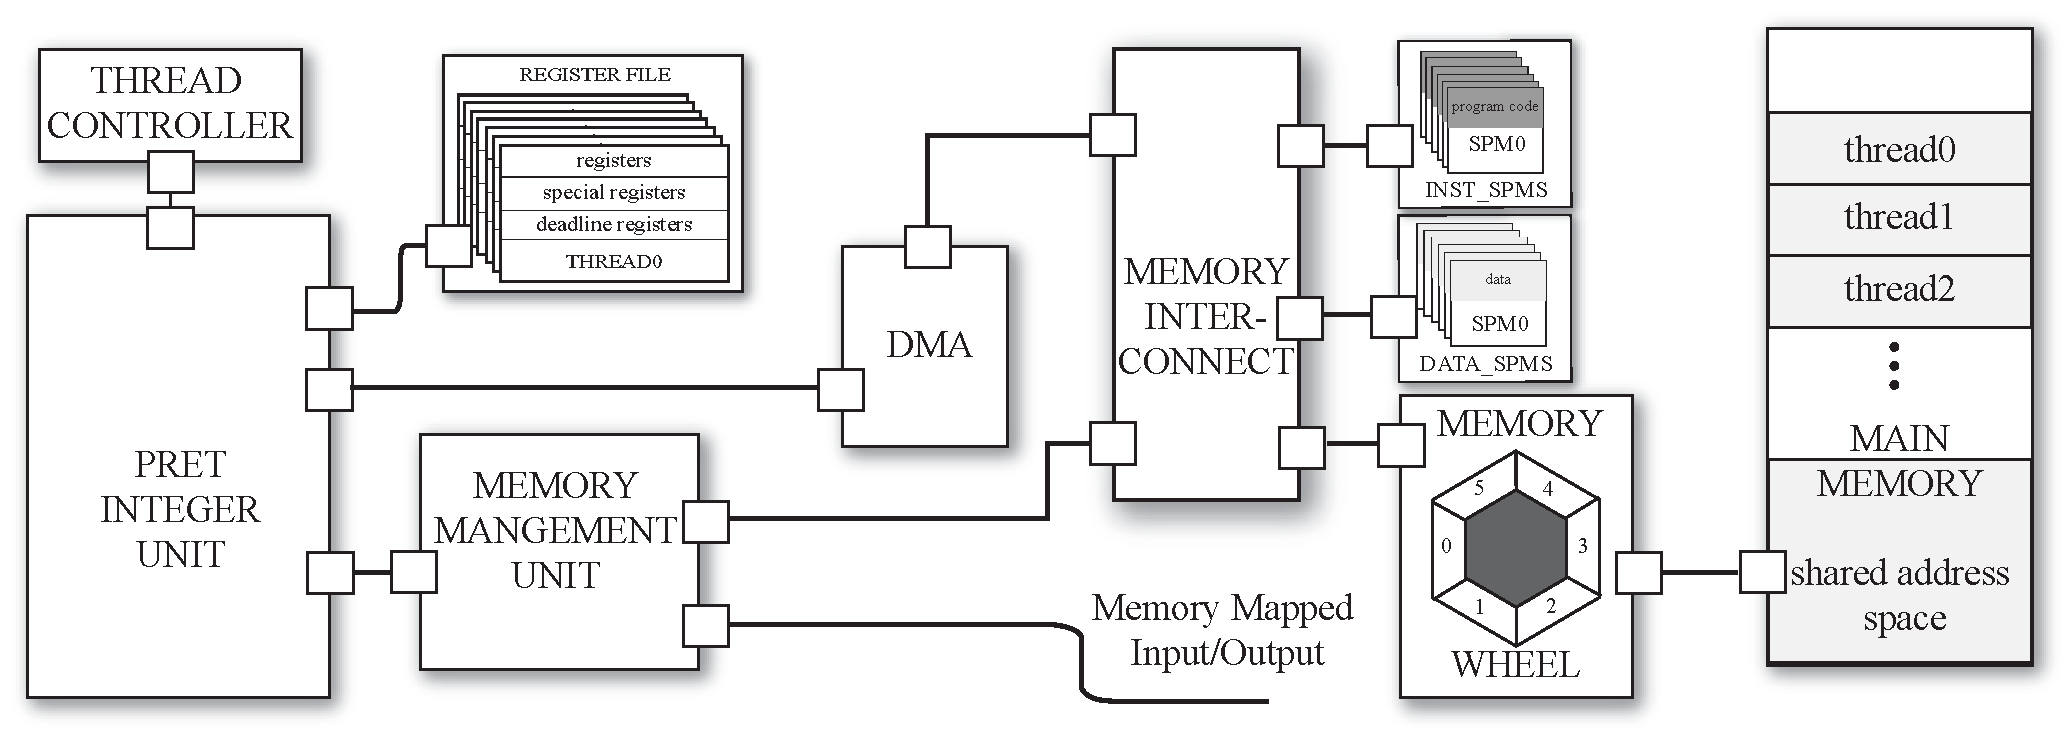
\includegraphics[width=\textwidth]{./images/top_arch.pdf}
%%   \caption{Unit Diagram for PRET Architecture. Reproduced with permission~\cite{pret_cases08}. }
%%   \label{fig:compview}
%%   \end{figure}

\subsection{A Precision Timed Architecture for Embedded Security}
The foundation of time-exploiting attacks exploits the uncontrollable timing variability introduced to programs by underlying the implementation of encryption algorithms.
Software implementations naturally introduce varying run times because of data-dependent control flow paths.
Modern computer architectures create unpredictable execution times by abstracting away hardware optimizations meant to improve average case performance.      
In this section we will present several features of PRET that bring \textit{controllability} over timing to software, eliminating the origin of the attacks.
We will discuss the software extensions that allow timing specification in programs, and the predictable architecture to comply with these specifications.
These two approaches cannot be separated.
A predictable architecture by itself would only ease the feasibility of an attack, and software timing specifications are meaningless if they cannot be met by the hardware. 
By combining both hardware and software solutions, we yield a timing predictable and controllable architecture. 
Thus, by design, PRET prevents leakage of any timing side-channel information, and eliminates the core vulnerability of time-exploiting attacks.

\subsubsection{Controlling Execution Time in Software}
It is extremely difficult to control and reason about timing behaviors in software, even with adequate understanding of the underlying architecture.
Current instruction-set architectures (ISA) have neglected to bring the temporal semantics of the underlying architecture up to the software level.
Thus, architecture designs have introduced clever techniques to improve on average case execution time of the instructions, at the expense of introducing variability in instruction execution time.
These architecture improvements are hidden to the software behind the abstraction of the ISA.   
%The difference in execution time for different paths of the program are often a result of optimizations to the program performance.
This proves to be costly in terms of security, because it uncontrollably leaks timing information which can correlate to the secret key.

In section~\ref{sec:programming_models} we introduce several ISA extensions that add time controlling behaviors to software. 
The extensions provide timing instructions that enable a programmer to have more control of execution time in software.
These instructions do not physically alter processor speed, or modify the execution time of instructions on the architecture.
Instead, they are meant to aid the programmer in dealing with timing variability from data-dependent control flow paths by allowing the programmer to interact with various execution time behaviors in software. 
This includes the ability to specify a desired execution time for code segments, and the ability to detect and handle situations when the execution time exceeds the desired amount.
Specifically in this context, the ability to enforce a minimum execution time for code segments proves extremely useful for mitigating the varying execution speeds exhibited by algorithms or code segments.  
We showed in section~\ref{sec:1dCFD} how the \emph{delay\_and\_set} instruction can be used to synchronize execution and communication of different nodes for an implementation of a real-time 1D-CFD simulation.  
Encryption algorithms can exhibit varying execution time behaviors depending on the bits of the encryption key.
The algorithm follows different execution paths if a particular bit in the key is set or not, allowing attackers to exploit this execution time variance to obtain the key.
By using the timing instructions provided by the PRET architecture, we can mitigate the effects of this, eliminating the exploit causing this timing  attack.  

At the expense of more programming effort, other solutions have been proposed to alter and pad the execution time of different execution paths~\cite{Kocher96timingattacks} to shield against the timing variability of the algorithm. 
At a glance it might seem that the timing instructions are a similar solution to these proposals, however, the principles are inherently different. 
While effective against certain time-exploiting attacks, existing solutions alter the underlying algorithm implementation in attempt to manually pad or distort the execution time. 
These solutions are not only algorithmically specific, but could lead to unnecessarily degrading of the performance of the encryption algorithms. 
The timing instructions, on the other hand, allow for a separation of concerns between the functionality and timing behavior of the code. 
The programmer can implement the correct functionality of the algorithm, then use timing instructions to regulate its timing behavior.
The subtle difference will be more apparent in section~\ref{sec:rtencrypt-results} when we show two different implementations of the RSA encryption that both use timing instructions to regulate execution time.
One implementation mimics existing execution time padding solutions, and the second implementation uses timing instructions to enforce an overall execution time of the RSA algorithm. 
We present performance comparisons and show that explicit timing control instructions could prove more beneficial than simple execution time padding.  

 %in the results section in section~\ref{sec:rtencrypt-results}. 
% The first implementation mimics the behavior of an existing execution time padding solution by forcing the execution time of all modular exponent operations, regardless of the bit value from the encryption key. 
% This solution leads the execution down the worst-case execution path for any encryption key, which we argue is unnecessarily degrading the algorithm performance.     
% Our second implementation uses statistical analysis on the run time of various input keys in encryption algorithms to determine the enforced execution time of the algorithm. 
% This leads to a modest performance improvement compared to the first approach, as the execution path is not forced down the worst-case path.

%We observe the normal distribution of execution times for the RSA encryption, and chose an execution time that covered roughly 97\% of the keys running in the RSA algorithm.    
%Without modifying the algorithm itself, the timing instructions regulated the execution time to   

%However, because these don't change architectural behavior, 
The timing instructions provide a method to control the timing behavior of a program in software.
However, they do not change the behavior of the underlying architecture.
If the underlying architecture makes the reasoning of execution time difficult, then these instructions become more difficult to use.
Timing instructions alone do not prevent attacks that exploit architectural designs to inject execution time variances~\cite{Percival05cachemissing,branchpredict} and obtain side-channel information. 
We argue that a \textit{predictable} architecture is also required to eliminate timing exploiting attacks.

\subsubsection{Predictable Architecture}
\paragraph {Pipeline}
% In order to improve instruction throughput and performance, modern processor architectures implement pipelines to execute multiple instructions in parallel.
% This requires handling of pipeline hazards, which are caused by dependencies in instruction sequences. 
% Conditional branches are the perfect example---the pipeline cannot fetch and begin executing the next instruction without knowing which instruction to fetch. 
% Since a conditional branch usually takes more than one cycle to resolve, the processor is forced to stall until the branch is resolved. 
% 
% Computer architects use clever speculative techniques to mitigate the effects of pipeline hazards and to substantially improve the average-case performance.
% For example, branch predictors are used to guess the next instruction needed by the processor for branches~\cite{Grunwald98confidenceestimation}.
% This allows the processor to execute instructions speculatively while rolling back only when needed. 
% %If the speculation is correct, there is no performance penalty, otherwise, the pipeline is flushed and a new instruction stream is fetched.
% While these speculative techniques improve the average-case performance, they introduce several side effects. 
%they result in computer architectures that are \textit{unpredictable}, and \textit{uncontrollable}. 
% \FIXME{Isaac: I find that it would be better to say that these architectures are unpredictable, which make cycle-counting and static prediction of execution times virtually impossible. The uncontrollability has two issues: 1) it's not possible to determine the execution times due to unpredictability, and 2) no method of allowing to do so either (no instructions)}
Modern processor architectures often use speculation techniques such as caches and branch predictors to improve average performance.
These create \textit{timing variations} in the program execution.  
Depending on the outcome of its speculation, the processor might need to discard the wrongly speculated work, and re-execute the correct instructions. 
Since these units are shared by all software processes concurrently running on the processor, the states of the speculation units are heavily dependent on the different interleaving of processes. 
This means that a process can unknowingly be affected by other processes, since the speculation state is shared between them~\cite{leethreads}.
This makes these units \textit{unpredictable}.
Because the goal of these speculation techniques is to improve program performance without effort from the programmer, the controls of these speculation units are concealed from the programmer, and cannot be directly accessed in software. 
Thus, these side effects result in \textit{uncontrollable} timing behaviors in the program.

Multithreaded architectures enable more opportunities to exploit the uncontrollable timing behaviors.   
Attackers exploit such architectures by running a spy thread that executes concurrently with a thread that implements the encryption algorithm.
This spy thread probes the components shared with the encryption thread~\cite{Percival05cachemissing,branchpredict} by forcefully occupying the shared units and observing when they are evicted by the encryption thread. 
The announcement of this vulnerability caused Hyper-Threading, Intel's implementation of simultaneous multithreading, to be disabled by default in some Linux distributions because of its security risks~\cite{hyperthreadharmfulsite}.
For general purpose applications, these side effects pose insignificant threats, but for security applications, the consequences are uncontrollable sources of side-channel information leakages.

%The PREcision Timed (PRET) architecture is a timing predictable architecture proposed for real-time embedded systems.
As discussed in chapter~\ref{section:pret_thread_pipeline}, PRET employs a thread-interleaved pipeline, a multithreaded pipeline that uses a predictable round-robin thread scheduling policy between the hardware threads every cycle.
The thread-interleaved pipeline eliminates the need for any data forwarding/bypassing logic, along with the need for hardware speculation units such as branch predictors.
Each individual hardware thread maintains their own copy of the processor state (program counter, general purpose registers, stack pointer, etc.), and each hardware thread runs independently with no shared state in the pipeline. 
Because of the simple and transparent thread-scheduling policy, each hardware thread gets dispatched in a predictable way that cannot be affected by other hardware threads. 
Thread-interleaved pipelines allow us to gain higher instruction throughput without the harmful side effects.
Most importantly, the hardware threads are temporally isolated, meaning that no threads can affect each others timing behavior. 
This prevents attackers from exploiting shared resources from the pipeline to initiate timing side-channel attacks.    

\paragraph{Memory System}
The memory system presents another opportunity for attackers to gain side-channel information.
The high clock speed of modern processors combined with the high latency to access main memory results in sometimes hundreds of cycles stalled when the processor needs to access the main memory.
On-chip fast access memories are used to bridge this access latency, creating a \emph{memory hierarchy}.
Caches are \textit{hardware-controlled} fast-access memories that predict and prefetch data from main memory based on temporal and spatial locality of data accesses from the processor.
If the cache control speculation is accurate, then access to data can complete in one cycle, and no stall in the pipeline is required.
However, when a misprediction occurs, data needs to be fetched from the main memory, causing a drastic difference in the access time~\cite{thiele:04:predictable}.
Caches abstract away the memory hierarchy and the access latency variation from the programmer by managing the cache contents in hardware.  
Because threads and processes share the same memory system, attackers can probe the memory access patterns of the encryption process by evicting shared cache lines and observing the timing variation the eviction causes~\cite{Percival05cachemissing}.
This is possible because the memory hierarchy is abstracted away from the programmer, resulting in \emph{uncontrollable} timing behaviors. 
%The cache states are manged in hardware, and shared by all threads and processes.   

PRET utilizes scratchpads memories (SPM) instead of caches in its memory hierarchy.  
SPMs are fast access memories controlled by software. 
% SPMs use less power and occupy less area~\cite{Banakar2002} because no speculation logic is needed. 
% SPMs occupy a distinct address space, which exposes the memory hierarchy to the programmer, instead of abstracting it away like caches.  
% The allocation of data between memory and SPM is done with explicit instructions, either at compile time by the compiler or manually by the programmer.
% This gives the software control over memory access latencies, and provides a predictable execution time of the program.
% The performance of SPMs vary based on the data access patterns of the application, but since the control is in software, it is possible to tune the allocation scheme to achieve even better performance than a generic cache for specific applications. 
% There are abundant ongoing research on allocation schemes and methods for optimizing the performance of SPMs~\cite{avissar2002oma,Bandyopadhyay06_AutomatedMemoryAllocationOfActorCodeDataBufferInHeterochronous,Patel:EECS-2008-115,Suhendra2005WCETSPM,compilerSPM}. 
% SPMs can be found in the Cell processor~\cite{cellproc}, which is used in Sony PlayStation 3 consoles, and NVIDIA's 8800 GPU, which provide 16KB of SPM per thread-bundle~\cite{8800gpu}.
% Although this comes at the cost of more programing effort, but it is not uncommon to see platform specific tuning of software for performance purposes. 
% For example, high performance parallel algorithms are often fine tuned to work on block sizes depending on the cache size and replacement policy of the platform, and re-tuned when running on different platform.
For security purposes, the scratchpad on PRET is configured to provide each hardware-thread a private scratchpad region so the scratchpad contents cannot be modified or monitored by spy threads on running another hardware thread.    
This prevents shared resource time-exploiting attacks on the fast access memory across hardware threads.
Even if an encryption process is sharing a hardware thread with another process, the contents of the scratchpad is controlled in software or statically compiled in by the compiler.
The thread managing supervisor code can manage the contents on the scratchpad before the processes are scheduled and unscheduled, preventing a spy process from affecting the execution time of the encryption process. 
Clearly, the edge that SPMs give over conventional caches is their \emph{controllability} in software.
This prevents unwanted timing side-effects from attackers and spy threads, even if the SPM is shared by software processes.
%If caches must be used, hardware additions to the cache
%Partition locked caches, which allows software processes to to lock cache lines which have proven successful against cache attacks~\cite{cachepartition}, can be implemented. 

Although no known attacks have exploited main memory access, typical DRAM controllers also result in variable memory access latencies, and are shared among all threads and processes within the system. 
A predictable DRAM controller is designed and interfaced with the thread-interleaved pipeline of PRET to provide predictable memory access latencies to all threads. 
The DRAM controller privatizes DRAM bank resources to remove bank conflicts and fully utilize bank level parallelism on the DRAM.  
Each hardware thread in the thread-interleaved pipeline is mapped to a privatized DRAM bank resource.
On the backend, the bank resources are accessed in a round robin order fashion, to remove temporal interference between accesses to the bank resources.
All memory accesses from the hardware threads are isolated from each other, removing any possibilities of cross-thread side-channel attacks from the shared memory controller.
The DRAM memory access latencies are decoupled from the data access patterns, thus, even processes on the same hardware thread that access the same bank resources cannot alter each others execution time in attempt to gain side-channel information.  
More details on the PRET DRAM controller is presented in section~\ref{sec:pret_dram_controller}.

We acknowledge the many efforts to counteract timing attacks with algorithm rewrites to control and balance the run time of the algorithm. 
These efforts, while successful, are ad-hoc, counteracting specific attacks without prevention of others.
Without tackling the origin of time-exploiting attacks, we believe that more exploits will eventually be discovered, attacking the \emph{uncontrollable} execution time variation caused by the shared resources of hardware or software control flow.  
The PRET architecture provides control of timing properties in software and a predictable architecture that with temporal isolation for its hardware threads.
PRET is impenetrable known attacks such as branch predictor attacks~\cite{Onur07predictingsecret}, cache attacks~\cite{Percival05cachemissing} or other attacks on the pipeline~\cite{2009-x86timing}.
More importantly, the predictable architecture design removes the root cause of time-exploiting attacks---the \emph{uncontrollable} timing variations caused by unpredictable hardware components or software control flows.     

\subsection{Case Studies}
\label{sec:rtencrypt-results}
In the following section we show the results of two encryption algorithms running on the cycle accurate simulator of the PRET architecture described in lickly et al~\cite{pret_cases08}.
Lickly et al.\cite{pret_cases08} introduced the first realization of the PRET architecture that implements the SPARC v8 instruction set.
It employs six threads on a six stage thread-interleaved pipeline, and also uses scratchpads for an expose memory hierarchy.
Programs are written in C and compiled using a standard gcc cross compiler from Gaisler research labs~\cite{GAISLER}.
Because the results of these experiments have yet to be ported to the newer PTARM, we present the original measurements obtained on the SPARC realization of the PRET architecture.  

The precision timed SPARC architecture implements a simple processor extension inspired by Ip and Edwards~\cite{ip2006processor} that adds timing instructions to the ISA.
To be consistent with the terminology used in~\cite{ip2006processor}, we call this instruction the \textit{deadline instruction}.
This deadline instruction has similar semantics to the \emph{delay\_and\_set} macro introduced in section~\ref{sec:programming_models}. 
It first ensures the previous deadline specified is met, then sets the deadline for the next instruction sequence.
The deadline instruction specifies time in the units of thread cycles, which are a thread's perceived cycle.
  
% The deadline instruction is used to load values into a special set of registers, called the \textit{deadline registers}. 
% In ~\cite{ip2006processor}, these registers are decremented each clock cycle in hardware, and act as hardware cycle counters. 
% Whenever the processor executes a deadline instruction, it first checks the corresponding deadline register's contents. 
% If it is zero, then the value specified in the instruction is loaded into the register, and the program continues. 
% If not, the processor replays this instruction until the value reaches zero. 
% Figure ~\ref{fig:timing_want} shows a simple illustration of what the deadline instructions look like.
% By enclosing instruction blocks within two deadline instructions, we can specify that the enclosing code block should run for x or y cycles.
% In ~\cite{ip2006processor}, this instruction was implemented for a single cycle processor. 
% PRET extended this instruction to be used in a multi-threaded pipeline architecture. 
% We will later show a more concrete example of how this instruction is extended for PRET.

% \begin{wrapfigure}[13]{l}{.4\textwidth}
%   \centering
%   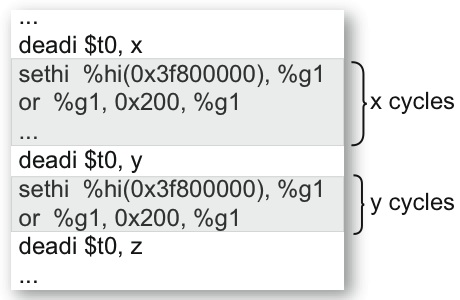
\includegraphics[scale=.7]{./figs/RTencrypt/timing_want.jpg}
%   \caption{A method to express timing requirement in software.}
%   \label{fig:timing_want}
% \end{wrapfigure}

%%Talk about the different in decrementing deadlines in PRET vs
%%original paper?
%This instruction allows a user to specify the execution time of the code enclosed within the deadline instructions. 


% \subsubsection{Timing instructions on PRET}
% 
% \begin{wrapfigure}[11]{r}{.4\textwidth}
% %\begin{SCfigure}
%   \centering
%   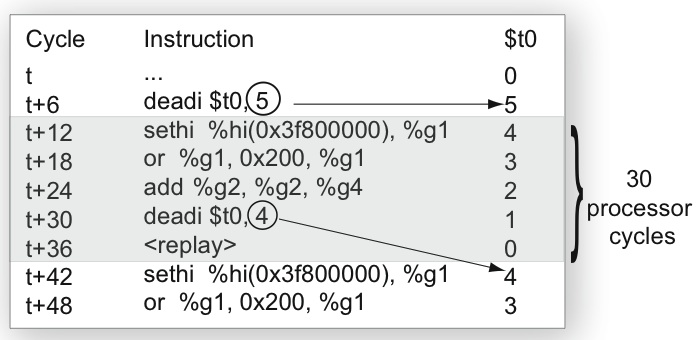
\includegraphics[scale=.53]{./figs/RTencrypt/timing_instructions.jpg}
%   \caption{A simple example using deadline instructions on PRET}
%   \label{fig:deadline}
% %\end{SCfigure}
% \end{wrapfigure}
% 
% Since PRET has multiple hardware threads, each hardware thread contains its own set of deadline registers, which are decremented every time an instruction from that thread is fetched into the pipeline.
% Specifically, PRET has six hardware threads, so each hardware thread's deadline registers are decremented every six processor cycles.
% Figure~\ref{fig:deadline} shows a concrete example of the execution of one thread on PRET using the deadline instruction.
% The three instructions enclosed between the deadline instructions take exactly 30 cycles to execute. 
% \textit{\$t0} shows the contents of deadline register 0. 
% The processor cycle is shown to the left of the instruction.
% When the first deadline instruction is executed, the instruction will simply load 5 into deadline register 0 and continue because the value of \emph{\$t0} is currently 0.
%  When the second deadline instruction is executed, since the value of \emph{\$t0} is not decremented to zero yet, this instruction will be replayed. 
% Only at \emph{t+36} cycles will the value 4 be loaded into deadline register 0.
% This ensures that the code enclosed will take 30 cycles to execute, as specified in the first deadline instruction. 
% We will show two real-world examples of using deadline instructions with encryption algorithms later in the case study section.

\subsubsection{RSA Vulnerability}

The central computation of the RSA algorithm is based primarily on modular exponentiation. 
This is shown in algorithm~\ref{alg:rsa}.
Of the inputs, $M$ is the message, $N$ is a publicly known modulus, and $d$ is the secret key.  
Depending on the value of each bit of $d$ on line 4, the operation on line 5 is either executed or not. 
This creates variation in the algorithm's execution time that is dependent on the key, as mentioned in \cite{Kocher96timingattacks}.

\begin{minipage}[h]{0.4\textwidth}
  \scriptsize
\begin{algorithm}[H]
\label{alg:rsa}
  \LinesNumbered
  \SetAlgoVlined
\KwIn{M, N, d = $(d_{n-1}d_{n-2} . . . d_{1}d_{0})$}
\KwOut{S = M$^{d}$ mod N}
S $\leftarrow$ 1 \\
\For{j = n - 1 $. . .$ 0} {
S $\leftarrow$ S$^{2}$ mod N \\
\If{d$_{j}$ = 1} {
S $\leftarrow$ S $\cdot$ M mod N
}
\textbf{return} S
}
\caption{RSA Cipher}
\end{algorithm}
\end{minipage}
\begin{minipage}[h]{0.6\textwidth}
  \scriptsize
\begin{algorithm}[H]
  \LinesNumbered
  \SetAlgoVlined
\KwIn{M, N, d = $(d_{n-1}d_{n-2} . . . d_{1}d_{0})$}
\KwOut{S = M$^{d}$ mod N}
S $\leftarrow$ 1 \\
\For{j = n - 1 $. . .$ 0} {
/* 110000 is 660000$\div$6 cycles, since deadline registers are decremented every 6 cycles.*/ \\
\textbf{dead(110000);}\\
 S $\leftarrow$ S$^{2}$ mod N \\
\If{d$_{j}$ = 1} {
S $\leftarrow$ S $\cdot$ M mod N
}
\textbf{dead(0)}; \\
\textbf{return} S
}
\caption{RSA Cipher with deadline instructions}
\label{alg:rsa_w_dead}
\end{algorithm}
\vspace{2mm}
\end{minipage}


%Our analysis of the algorithm demonstrated that a significant portion of the variation in the algorithm's execution time could be attributed to the branch in the loop above.  
When the reference implementation of RSA (RSAREF 2.0) was ported to the precision timed SPARC architecture, single iterations of the loop varied in execution time almost exclusively due to the value of d$_{j}$, which is the j$^{th}$ bit of the key. 
The triangle points in figure \ref{fig:modexp} show the measured run time of each iteration in the for loop (lines 2--6) in algorithm \ref{alg:rsa}. 
Each iteration took approximately either 440 or 660 kilocycles, with very little deviation from the two means.
As a simple illustration, we can fix the execution time of each iteration in software  by adding deadline instructions in the body of the loop as shown in algorithm~\ref{alg:rsa_w_dead}. 
When enclosed with deadline instructions, the execution time of each iteration is uniform, and the bimodality of the execution time is completely eliminated. 
The x points in figure \ref{fig:modexp} show the measured time of each iteration after adding deadline instructions; they are simply a straight line.

\begin{figure*}[h]
\centering
\subfigure[Run time of Modular Exponent operation] {
  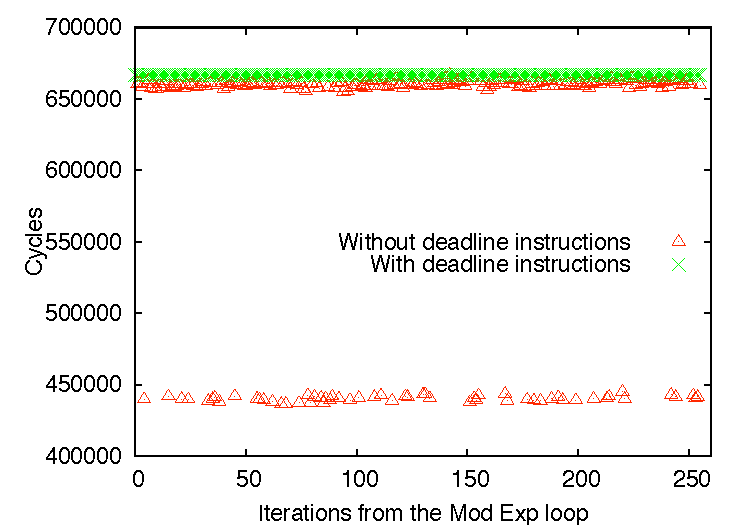
\includegraphics[width=0.48\textwidth]{./figs/RTencrypt/ModExp.pdf}
  \label{fig:modexp}
}
%\quad
\subfigure[Run time of RSA operation]{
  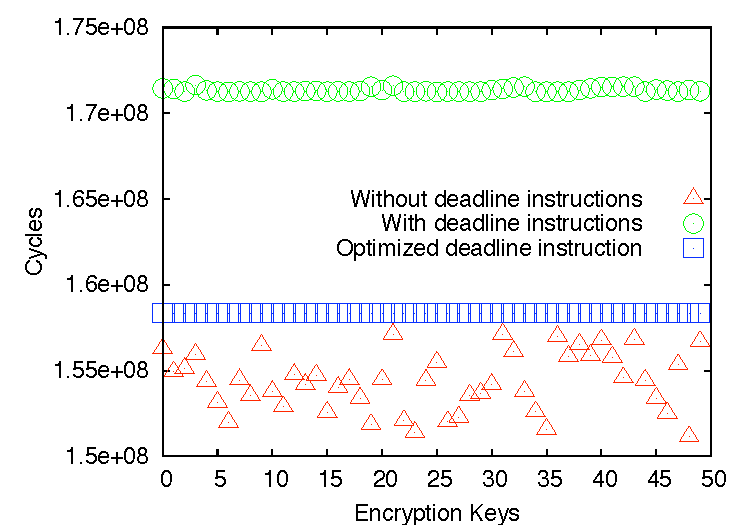
\includegraphics[width=0.48\textwidth]{./figs/RTencrypt/RSA.pdf}
  \label{fig:rsa}
}
\caption{RSA Algorithm}
\end{figure*}



%We see that all iterations took exactly the same amount of time. 
%These results seem obvious, but reveal the power of software-controlled execution time. 
%Now algorithms that require constant run time can easily be specified in software.  
%Additionally, placing deadline instructions in this loop completely eliminates the vulnerability mentioned in Kocher's\cite{Kocher96timingattacks} classic timing attack paper. 
We observe the large-scale effect of this small change on the whole encryption in figure~\ref{fig:rsa}, where RSA was run fifty times using randomly generated keys.
Without the deadline instructions (triangle points), different keys exhibit significant diversity in algorithm execution time.  
With the deadline instructions added within the modular exponentiation loop (circle points), the fluctuation is dramatically reduced to almost none. 
The remaining small variations result from code that is outside of the modular exponentiation loop, which is not influenced by the actual key.
From figure ~\ref{fig:rsa} we can see that this small variation  is not significant enough to correlate the total execution time and the key.  

% Although it seems we could have achieved a similar effect if we simply forced the algorithm to carry out the extra operation every iteration, there is a subtle difference.
% As mentioned in~\cite{Kocher96timingattacks}, always carrying out the extra multiplication operation does not make the implementation run at constant time, and timing characteristics from the squaring operation can still be exploited. 
% However, constant run time is guaranteed for code blocks enclosed within the deadline instructions, which in our case includes both the multiplication and squaring operations for each iteration.
% This simple example demonstrates the difficulty of controlling execution time using software techniques, and how straightforward it is to do so using deadline instructions. 
% This is a simple example demonstrating the concept of the deadline instruction.  
% However, for more complex algorithms, the changes required to create constant execution time might not be as obvious.
% In those situations, deadline instructions provide a straightforward mechanism to control the execution time of the algorithm.

%Although this method makes RSA secure against timing attacks, it does incur a notable performance penalty because we always run the algorithm near its worst-case execution time.
Without explicit control over timing, any attempt to make an algorithm run at constant time in software would involve manual padding of conditional branches.
This forces the algorithm to run at the worst-case execution time, similar to what we have showed.
Although this makes the encryption algorithm completely secure against time-exploiting attacks, this method is not adopted in practice because of the overhead.
Nevertheless, with control over execution time, we will show that running encryption algorithms in constant time does not necessarily require it to run at the absolute worst-case execution time.

%smarter techniques with deadline instructions can be used to achieve better performance while still being secure.
%Although the vulnerability is removed, readers will have noticed that an overhead was induced in this simple example. 
%The reason for the overhead is apparent, and mentioned above. 
% This overhead is not a result of the deadline instruction itself. 
% When we added the deadline instructions to the inner most loop of the modular exponentiation, in order to completely remove the vulnerability from RSA, we set the execution time of each loop iteration to always equal the execution time as if the extra operation was carried out. 
% As a result, the overall execution time will be the worst case execution time of the algorithm, as if our key was all bits of 1. 
% That is the overhead we see in figure~\ref{fig:rsa}. 
% This solution is effectively the same as timing equalization \textcolor{red}{(FIXME: add citation [do we really need one? or is this where a paper that talks about what timing equalization is would go?])} of algorithms, which now require little effort because timing can be controlled in software. 
\subsubsection{An Improved Technique of using Deadline Instructions} 

It is expected that the distribution of RSA run times will be normal over the set of all possible keys~\cite{Kocher96timingattacks}. 
Figure~\ref{fig:distro} shows the run time distribution measured for one thousand randomly generated keys. 
A curve fitting yields  a bell shaped curve formed from the run time distribution of all keys.
This means that the execution time of approximately 95\% of the keys will be within $\pm$2 standard deviations of the mean, and the worst-case execution time will be an outlier on the far right of this curve. 
Our previous example fixed the execution time of all keys to be \textit{roughly} at this far right outlier.
An improved technique capitalizes on this distribution of run times to improve performance.

First, instead of enclosing the loop iterations of the modular exponentiation operation, we enclose the whole RSA operation with deadline instructions. 
Now the deadline instructions are used to control the overall execution time of the RSA operation.
Note that we could have done this for the previous example as well to fix the execution time to be \textit{exactly} the worst-case, always. 

\begin{wrapfigure}[16]{r}{.45\textwidth}
%\begin{SCfigure}
  \centering
  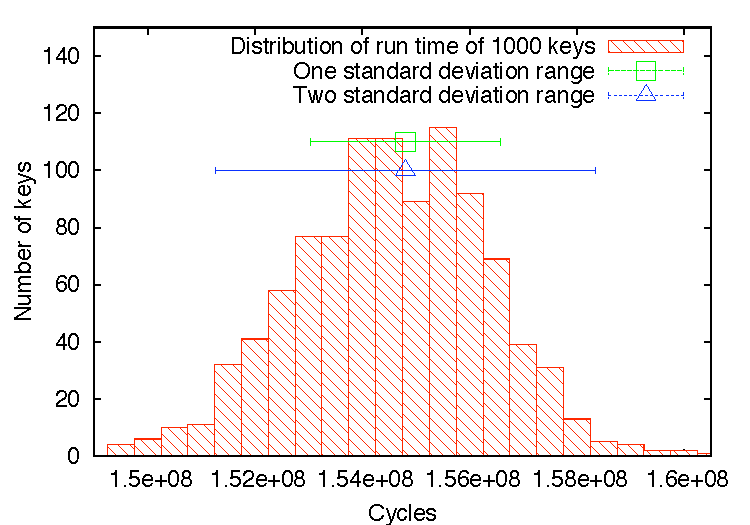
\includegraphics[scale=.60]{./figs/RTencrypt/Distro.pdf}
  \caption{Run time distribution of 1000 randomly generated keys for RSA}
  \label{fig:distro}
%\end{SCfigure}
\end{wrapfigure}

For RSA, key lengths typically need to be longer than $512$ bits to be considered cryptographically strong~\cite{redhatadminguide}. 
This gives roughly $2^{512}$ possible keys, which is far more than needed for most applications.
Suppose we are able reduce the key space the application covers---instead of using $100\%$ of the keys, we refine our encryption system to only assign $97\%$ of all possible keys. Namely, the subset of keys whose RSA execution times fall on the left of the $+2$ standard deviation line on the curve.
Statistically, the keys that lie outside of $\pm 2$ standard deviation are the least secure keys, since it is easier for time-exploiting attacks to distinguish those keys. 
%Then, we can reduce the value specified in the deadline instruction enclosing the whole RSA operation instead of using the absolute worst-case execution time pushed up by the far right outlier.
By doing so, we reduce the execution time of the encryption algorithm because we know that keys that are right-side outliers will not be used. 

With timing control in software, we can take advantage of this information by simply reducing the value specified in the deadline instructions enclosing the whole RSA operation. 
The square points in figure~\ref{fig:rsa} show the results of using deadline instructions in this way. 
We re-ran the same fifty keys from the previous section, and enclosed the whole operation with deadline instructions that specified the run time at +2 standard deviations from the bell curve we obtained.
We can see that, compared to the previous results that fixed the execution time of each key to take  the worst-case time (circle points), we clearly reduced the overhead while still running in constant time. 
By taking the run time difference between executions with and without deadline instructions, we obtain the overhead introduced for each of the keys with run time below 2 standard deviations (97.9\% of keys in our case). % within the one thousand key set in our experiment. 
This calculation reveals that by merely reducing the key space by 3\%, running the encryption with optimized deadline instructions only introduced an average overhead of $2.3\%$ over all the keys we measured. 
All this while still being completely immune to time-exploiting attacks.
This is virtually impossible to achieve without explicit timing control, which illustrates the value of decoupling timing control and functional properties of software. 

%When running on PRET, we measured an average overhead of $11\%$ over the one thousand keys in the when we controlled the execution time of each iteration within the modular exponentiation operation.


\begin{figure*}[h]
\centering
\subfigure[Distribution of 1000 DSA keys ] {
  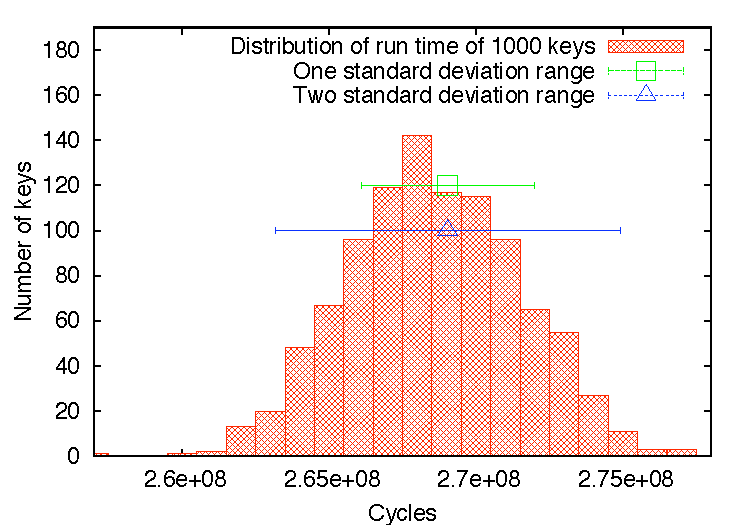
\includegraphics[width=0.48\textwidth]{./figs/RTencrypt/DSA_Distro.pdf}
  \label{fig:dsamodexp}
}
%\quad
\subfigure[Run time of 100 DSA operations]{
  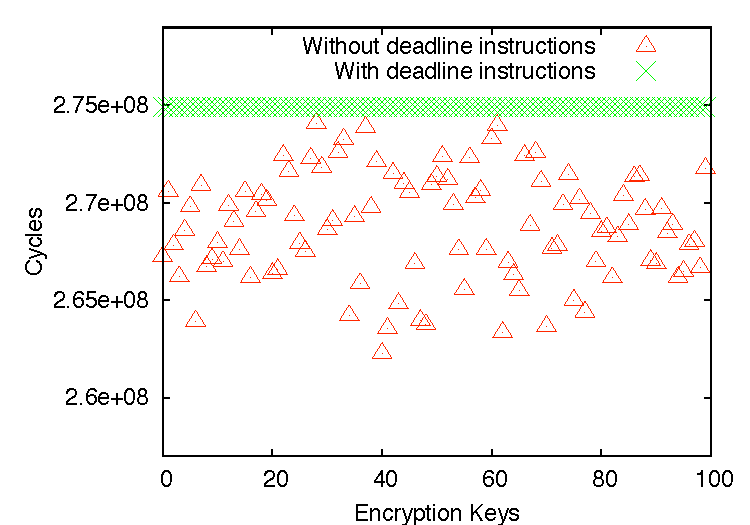
\includegraphics[width=0.48\textwidth]{./figs/RTencrypt/DSA.pdf}
  \label{fig:dsa}
}
\caption{Digital Signature Standard Algorithm}
\end{figure*}

\subsubsection{Digital Signature Algorithm}
Kocher's~\cite{Kocher96timingattacks} original paper mentioned that the Digital Signature Standard~\cite{dss} is also susceptible to timing attacks. 
Thus, to further illustrate our case, we port the Digital Signature Algorithm from the current OpenSSL library (0.9.8j) onto the precision timed SPARC architecture.
We use the same method mentioned above to secure this implementation on PRET.
Figure~\ref{fig:dsamodexp} shows the distribution of DSA run time for one thousand keys. It also shows a normal distribution.
Then, we randomly generate another one hundred keys, and measure the run time with and without deadline instructions, which we show in figure~\ref{fig:dsa}.
We can clearly observe that the run time with deadline instructions is constant, and any time-exploiting attack is not possible. 

%we can set different values for the deadline instruction depending on the application's needs to yield a balance between security and performance. 
% Another possible use of deadline instructions is to implement execution time blinding. 
% We can set the execution time  of the encryption operation to be a truly random value between $\pm$2 standard deviations of the total run time. 
% Whenever the value of the deadline instruction is less the actual run time of the algorithm, the algorithm will take its normal execution time. 
% However, if the value of the deadline instruction is more than the run time, then the algorithm will run at the time specified by the deadline instruction. 
% Since the deadline instruction value is random, it detaches the correlation between the key and the run time of the encryption. 
% This can also improve the average performance.

%Simply by running on PRET, RSA is not only immune to cache attacks and branch predictor attacks, both of which can be significant dangers to RSA\cite{branchpredict,Percival05cachemissing}, but also to potential unknown timing attacks targeting the unpredictability of the architecture. 

Currently, we do not know of any work that correlates the key value with run time for different encryption algorithms. 
However, with the ability to control execution time in software, such a study would be extremely valuable.
Figures~\ref{fig:distro} and~\ref{fig:dsamodexp} show that RSA and DSA follow a normal distribution.  
Thus, from the algorithm, we postulate that by simply counting the $1$ bits in the key should be sufficient to distinguish the $95\%$ of secure keys before assigning. 
Note that no change to the encryption algorithm itself is needed, but only the key assignment process.
Since we can adjust the execution time in software, we can tune the performance of each application based on the application size, key bit length and performance needs.
All this can be done while maintaining complete immunity against time-exploiting attacks.

Note that there are several other software techniques specific to encryption algorithms that successfully defend against timing attacks. 
Our work does not lessen or replace the significance of those findings.
Instead, we can use traditional noise injection defenses on PRET as well.
For example, if reducing the key space is not possible for some applications running RSA then RSA with blinding can be ran on PRET. 
By simply running on PRET, the encryption algorithm is also secure against shared hardware resource attacks such as caches, and branch predictors. 
Other encryption algorithms that do not have software techniques or solutions readily available to counteract timing attacks can easily use the deadline instructions provided by PRET to achieve security against timing attacks.

% \section{Future Work}
% While a deadline instruction set for the worst case execution time bestows complete immunity to timing attacks, it also places overhead on virtually every execution, which may be substantial depending on the application.  Lowering the minimum time, even randomly, gives some information to an attacker, especially if there is no limitation on the number of executions the attacker may observe.  A mathematical examination of the risk involved in a reduced execution time would enable the programmer to decide what tradeoff of risk and execution delay was appropriate for the application, or appropriate in general.  For example, reducing the potential key space to a tenth of all possibilities would most likelyside-channel be an acceptable trade for faster execution, while reducing it to a billionth of all possibilities probably would not be acceptable.

% On another note, the PRET architecture as it stands is vulnerable to power attacks.  By doing very little and drawing less power while waiting for deadlines to expire, timing attacks are basically converted into a subset of power attacks.  This is unacceptable for consumer applications such as set-top boxes, where power draw can be easily measured.  Modifying the architecture to spend energy while waiting would prevent such attacks.  Depending on the implementation of the power-draining system, it might even be extended to prevent most other power attacks as well by adding another power sink to that required for useful work.

\subsection{Conclusion and Future Work}
Side-channel attacks are a credible threat to many cryptosystems.  
They exist not just because of a weakness in an algorithm's mathematical underpinnings, but also from information leaks in the implementation of the algorithm. %The inability to control timing properties is what directly leads to side channel attacks.
In particular, this work targets time-exploiting attacks, and lays out a means of addressing what we consider the root cause of such attacks: the lack of \textit{controllability} over the timing information leaks.
%Although numerous efforts have been put to discovering and counteracting these attacks, it seems that only more vulnerabilities are being discovered. 
% Without secure hardware, software cannot be considered truly secure.  
% Some stopgap measures are implementable in software, but rarely are they a guaranteed fix.
%that originate from the \textit{unpredictability} of the underlying hardware architecture.
As an architecture founded on predictable timing behaviors, PRET provides timing instructions to allow timing specifications in software. 
In addition, PRET is a predictable architecture that removes timing interference between threads through a thread-interleaved pipeline, scratchpad memories, and a predictable DRAM memory controller.
This eliminates the shared states in the architecture that create uncontrollable timing interference, exploited by the attackers. 
Through a combination of hardware and software techniques, PRET gives control over the timing properties of programs, which effectively eliminates time-exploiting attacks. 

We demonstrate the application of these principles to known-vulnerable implementations of RSA and DSA, and show that PRET successfully defends against time-exploiting attacks with low overhead. 
Our work does not undermine the significance of any related work, which have mostly been specific to certain attacks.
PRET does not target a specific encryption algorithm, because it can be used in combination with these partial solutions on specific encryption algorithms, as well as provide a complete defense for other encryption algorithms that are less researched upon.

% Besides time-exploiting attacks, there are other side-channel attacks that are legitimate threats to encryption algorithms such as power, and fault attacks.
% We plan to continue to investigate PRET's effectiveness in defending against them. 
% We conjecture that the thread-interleaved pipeline used in PRET can potentially help defend against power attacks because the power measured from the processor now includes significant interference from the execution of other hardware threads in the architecture.  
%Currently, PRET is only implemented as a software simulator, but as PRET moves to FPGA implementations, we can further evaluate its effectiveness in defending against power attacks.
%If our conjecture is correct, then PRET with fault tolerant techniques could potentially be a complete solution against several major side-channel attacks.  